\documentclass{article}
\usepackage{amsfonts}
\usepackage{graphicx}

\title{A vision-based approach to Quadcopter detection and trajectory interception}
\author{Patricio Lankenau}
\date{May 4, 2014}

\begin{document}
\maketitle

\begin{abstract}
Our contribution is a vision-based approach to Quadcopter detection and trajectory interception.
We achieved visual recognition of the ball and quadcopter using a filtered Hough circle transform.
Furthermore, we achieved the trajectory prediction by implementing a least-squares regression.
\end{abstract}

\section{Related Work}

\section{Vision-based approach to detecting a ball}

Our original idea was to use a kinect to be able to detect a ball in 3D space, which would give
us the ability to predict where the ball is within a room. However, we hit our first obstacle
when we tried to interface with the kinect. The current state of drivers and interfaces that
are open source and linux compatible is a mess. We experimented with NI, freenect, and openCV\@.
And although we got it working in all three, we decided to use openCV because of it requires less
dependencies and is easier to develop with.

It was also at this point that we decided that we were going to have to narrow the scope of our
research if we were to get anything done in such a short span of time. We decided to reduce the
search space from $\mathbb{R}^3$ to $\mathbb{R}^2$, essentially operating on a 2D crossection of
the 3D world. This simplifying assumption allows us to only worry about points in $\mathbb{R}^2$
which makes everything else easier. Unfortunately, this decision came at a cost: we would no
longer be able to gather depth information on points (essentially using the kinect as a regular
camera). 

Once we were able to get a video feed from the camera, our next step was to detect the ball. Our
first thought was to use a Hough Circle Transform, but our naive implementation was unreasonably
slow. After consulting people well-versed in the field, they recommended that we detect the ball
using colored blob detection instead of HCT\@. We like the color idea, but were happy with HCT so
we decided to use color detection to filter out non-important colors in the image and then
performing HCT on the result.

In order to accurately filter the color we were interested in, we decided to concert the original
RGB image into a different colorspace. We experimented with various colorspaces, but chose to
convert to HSV (Hue, Saturation, Value). The advantages of switching to HSV is that we can filter
out a range of hues to get variations of a color. Filtering out in such a manner would not be
possible in the traditional RGB space since hues span across all three values. Once we managed
to convert the image to HSV, we apply a threshold to convert the desired color to white, and
everything else to black. This essentially outputs a binary imagine that we then feed to the
Hough Circle Transform. This proved to be very efficient and fast. We tested recognizing a ball
with varying amounts of noise and were constantly processing at around 25 frames per second.

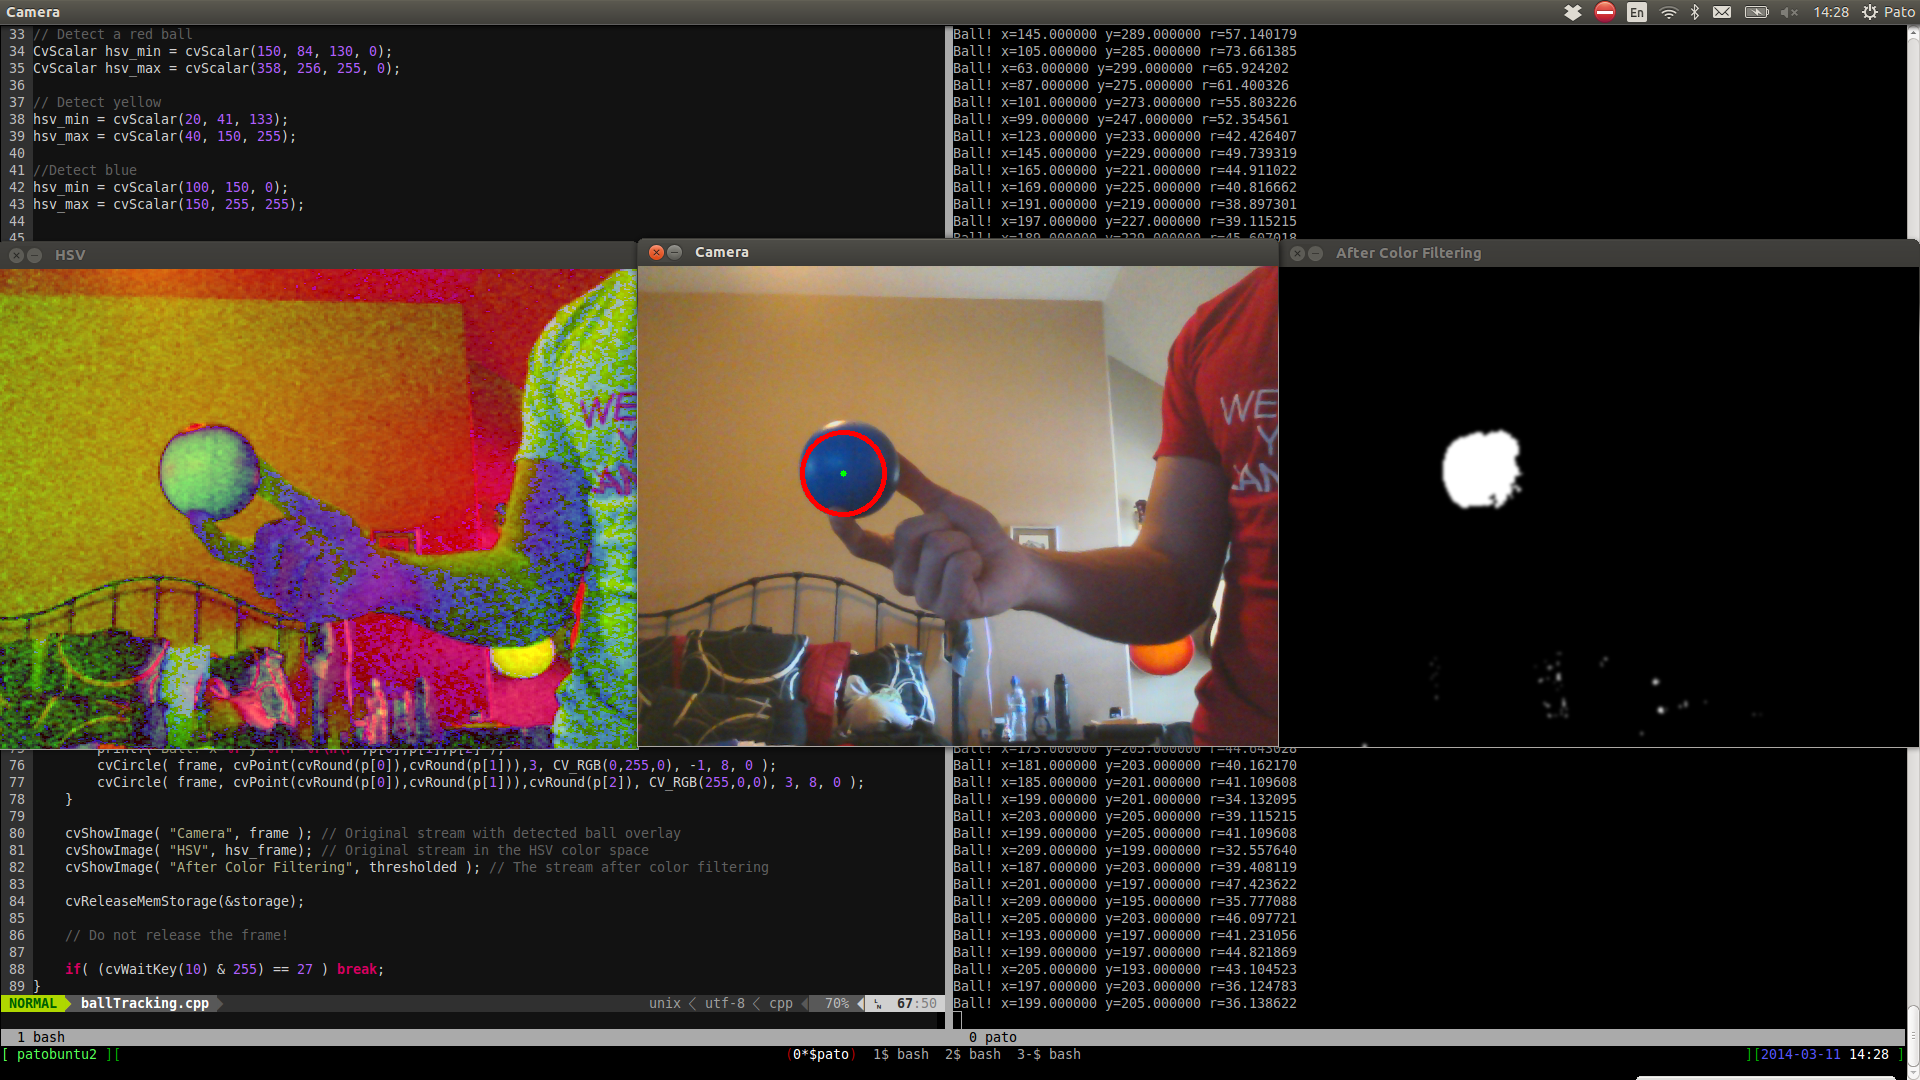
\includegraphics[scale=0.15]{../images/DetectingBlue.png}

Our final implemention of the recognition takes a video feed from either a webcam or kinect
and overlays circles whereever it detects a ball. We also show the intermediate steps of conerting
to HSV and the image after it has been thresholded.

\section{Trajectory prediction using least-squares regression}

\section{Quadcopter control}

\section{Putting it all together}

\section{Further work}

\end{document}
